\documentclass{beamer}
\usepackage[utf8]{inputenc}

\usetheme[progressbar=frametitle]{metropolis}

\usepackage{appendixnumberbeamer}

\usepackage{booktabs}
\usepackage[scale=2]{ccicons}

\usepackage{xspace}
\newcommand{\themename}{\textbf{\textsc{metropolis}}\xspace}

\usepackage{amsthm}
\usepackage{amssymb}
\usepackage{amsmath}
\usepackage{hyperref}
\usepackage{caption}
\usepackage{mathrsfs}
\usepackage{blkarray}
\usepackage{mathtools}
\usepackage{float}

\usepackage{natbib}
\setcitestyle{authoryear}

\usepackage{graphicx}

\usepackage{tikz}
\usetikzlibrary{calc, automata, chains, arrows, arrows.meta, graphs, graphs.standard, matrix, positioning, scopes}

\makeatletter
\tikzset{join/.code=\tikzset{after node path={%
\ifx\tikzchainprevious\pgfutil@empty\else(\tikzchainprevious)%
edge[every join]#1(\tikzchaincurrent)\fi}}}
\makeatother
\tikzstyle{labeled}=[execute at begin node=$\scriptstyle,
   execute at end node=$]
   
\theoremstyle{definition}
\newtheorem{defn}[theorem]{Definition}

\newcommand{\R}{\mathbb{R}}
\newcommand{\Rs}{\mathcal{R}}
\newcommand{\Gs}{\mathcal{G}}
\newcommand{\Cs}{\mathcal{C}}
\newcommand{\Q}{\mathbb{Q}}
\newcommand{\A}{\mathcal{A}}
\newcommand{\F}{\mathcal{F}}
\newcommand{\E}{\mathcal{E}}
\newcommand{\M}{\mathcal{M}}
\newcommand{\N}{\mathbb{N}}
\newcommand{\Z}{\mathbb{Z}}
\newcommand{\Zs}{{\{0,1\}^\mathbb{Z}}}
\newcommand{\I}{\mathcal{I}}
\newcommand{\D}{\mathcal{D}}
\newcommand{\B}{{\mathcal{B}_{\mathbb{R}}}}
\newcommand{\BU}{{\mathcal{B}_{[0,1]}}}
\newcommand{\loc}{L_{\text{loc}}^1}
\newcommand{\powset}{\mathcal{P}}
\newcommand{\outm}{\mu^{*}}
\newcommand{\cdict}{\Rightarrow\!\Leftarrow}
\newcommand{\Var}{\operatorname {Var}}

% X_1, ..., X_n
\newcommand{\Xn}{\ensuremath{X_1,\ldots,X_n}}
\newcommand{\xn}{\ensuremath{x_1,\ldots,x_n}}

\title{Phase-Type Distributions for Finite Interacting Particle Systems}
\subtitle{Master's Thesis}
\author{Stefan Eng\\
    Advisor: Jeff Steif
}
\institute{Göteborgs Universitet}
\date{June 9, 2020}

\begin{document}

\maketitle

\begin{frame}{Table of contents}
  \setbeamertemplate{section in toc}[sections numbered]
  \tableofcontents%[hideallsubsections]
\end{frame}

\section{Background}

\begin{frame}{(Finite) Interacting Particle Systems}
  \begin{figure}[H]
  \centering
    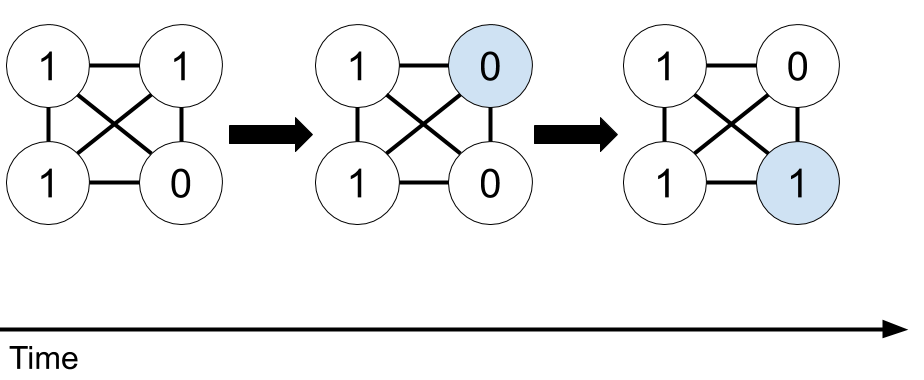
\includegraphics[width=.8\textwidth]{figures/ips_overview_transitions.png}
    \caption{An interacting particle system on a finite complete graph with 4 nodes}
\end{figure}
\end{frame}

\begin{frame}{Background}
A random variable $N$ is \textbf{geometrically distributed} with parameter $p \in (0,1]$ if $N$ is a non-negative integer random variable with probability mass function
$$
P(N = n) = (1 - p)^{n - 1} p
$$
for $n \in \{1,2,\ldots\}$.

A random variable $X \in [0, \infty)$ is \textbf{exponentially distributed} with rate $\lambda$ if it has a probability density function
$$
f(x; \lambda) = \begin{cases}
    \lambda e^{-\lambda x} & x > 0\\
    0 & x \leq 0
    \end{cases}
$$
\end{frame}

% \begin{frame}{Discrete Markov Chain}

% A stochastic process $(X_n)$ with countable or discrete state space $S$ is a (discrete) \textbf{Markov chain} if
%     $$
% P(X_{n + 1} = s | X_n = x, \ldots, X_0 = x_0) = P(X_{n + 1} = s | X_n = x)
% $$
% for all $n \geq 1$ and $s, x, x_{n-1}, \ldots, x_0 \in S$.

% and \textbf{time homogeneous} if
% $$
% P(X_{n + 1} = j | X_n = i) = P(X_{1} = j | X_0 = i)
% $$
% \end{frame}

\begin{frame}{Continuous-time Markov Chain}
The process $(X(t))$ is a \textbf{continuous-time Markov chain} (CTMC) with index set $\mathbb T$ (assumed to be $[0, \infty)$) and finite or countable state space $S$ if
$$
P(X(t_n) = j | X(t_{n - 1}) = i_{n-1}, \ldots, X(t_1) = i_{1}) = P(X(t_n) = j | X(t_{n - 1}))% = i_{n - 1})
$$
for all $t_1, \ldots, t_n \in \mathbb T$, with $t_1 < \cdots < t_n$ and $i_1,\ldots, i_{n - 1}, j \in S$.
\end{frame}

\begin{frame}{Continuous-time Markov Chain}
% Assuming the CTMC is in state $i$ at time $t$, the probability of moving to state $j$ in time $h$ for $h \to 0$ is given by
% $$
% P(X_{t + h} = j | X_{t} = i) = \begin{cases}
%     i \not = j & q_{ij} h + o(h)\\
%     i = j & 1 + q_{ii} h + o(h)
% \end{cases}
% $$

% A function $f$ is $o(h)$ as $h$ goes to 0 if 
% $$
% \lim_{h \to 0} \frac{f(h)}{h} = 0
% $$
\begin{itemize}
    \item The \textbf{infinitesimal generator matrix} $Q$, of $(X(t))$ with finite or countable state space $S$ is an $|S| \times |S|$ matrix.
    \item The elements $q_{ij}$ of $Q$ denote the rate departing from i and arriving in state j.
    \item Diagonal elements are defined as
    $$
    q_{ii} = - \sum_{j \not = i} q_{ij}
    $$
    \item If we are in state $i$ then the chain remains in state $i$ for an exponentially distributed time with rate $-q_{ii}$ before changing to another state $j$.
\end{itemize}


% with probability $-\frac{q_{ij}}{q_{ii}}$.
\end{frame}

\begin{frame}{Embedded Markov Chain}
\begin{itemize}
    \item Let $(X_t)$ be a continuous-time Markov chain with infinitesimal generator matrix $Q$
    \item Let $Y_n$ be the position of the $n$th jump of the process $(X_t)$ with $Y_0$ the initial state of the chain $(X_t)$
    \item This discrete-time Markov chain $(Y_n)$ is called the \textbf{embedded} (discrete) Markov chain of the process $(X_t)$.
    \item When $S$ is finite we have that the transition probability from state $i$ to state $j$ is
    $$
    P(Y_{n} = j | Y_{n - 1} = i) = -\frac{q_{ij}}{q_{ii}}
    $$
    if $q_{ii} \not = 0$
\end{itemize}
\end{frame}

% \begin{frame}{Example State space diagrams}
%     \begin{figure}[H]
%     \centering
%   \begin{tikzpicture}[start chain = going right,
%   -Triangle, every loop/.append style = {-Triangle}]
%   \node[state, on chain]  (2) {2};
%   \node[state, on chain]  (1) {1};
%   \node[state, on chain]  (0) {0};

%   \draw (2) edge[bend left] node[yshift=3mm]{$1$} (1);
%   \draw (1) edge[bend left] node[yshift=-3mm]{$\mu$}(2);
%   \draw (1) edge[left] node[xshift=3mm, yshift=-3mm]{$\lambda$} (0);

% \end{tikzpicture}
%     \caption{Rates for a continuous time Markov chain on $S = \{0,1,2\}$}
% \end{figure}

% \begin{figure}[H]
%     \centering
%   \begin{tikzpicture}[start chain = going right,
%   -Triangle, every loop/.append style = {-Triangle}]
%   \node[state, on chain]  (2) {2};
%   \node[state, on chain]  (1) {1};
%   \node[state, on chain]  (0) {0};

%   \draw (2) edge[bend left] node[yshift=3mm]{$1$} (1);
%   \draw (1) edge[bend left] node[yshift=-3mm]{$\frac{\mu}{\mu + \lambda}$}(2);
%   \draw (1) edge[left] node[xshift=3mm, yshift=-3mm]{$\frac{\lambda}{\mu + \lambda}$} (0);

% \end{tikzpicture}
%     \caption{Embedded Markov chain}
% \end{figure}
% \end{frame}

% \begin{frame}
%     \begin{theorem} \label{thm:geom_sum_exp}
%     Let $N$ be geometrically distributed ($N \in \{1,2,\ldots\})$ with probability of success $p$ and $X_1,X_2,\ldots$ i.i.d and independent of $N$ with each $X_i$ exponentially distributed with rate $\lambda$.
%     Then,
%     $$
%     S = \sum_{i = i}^N X_i
%     $$
%     has an exponential distribution with rate $p \lambda$.
%     \end{theorem}
% \end{frame}

\begin{frame}{Markov Chain Projection/Lumping}
\begin{itemize}
    \item Assume that we have a Markov chain $(X_t)$ with state space $S$ with generator $Q$
    \item Let $T = \{t_1, t_2, \ldots\}$ be partition of $S$.
    \item For any $x,x' \in t_i$ if
    $$
    {\displaystyle \sum _{y \in t_{j}}q(x,y)=\sum _{y \in t_{j}}q(x',y),}
    $$
    then $(X_t)$ is lumpable with respect to $T$.
    \item We refer to this new CTMC with state space $T$ a \textbf{projection}
\end{itemize}
% Let $(X_n)$ be a discrete-time Markov chain with state space $\Omega$ and transition matrix $P$.
% Let $\sim$ be an equivalence relation on $\Omega$ and denote the equivalences classes as $\Omega' = \{[x]: x \in \Omega\}$.

% If $x \sim x'$ implies that $P(x,[y]) = P(x', [y])$ (where $P(x,A)$ is probability that the chain moves in one step to one of the states $y \in A$ from $x$) then $([X_n])$  is a Markov chain.
% The state space is the equivalence classes $\Omega'$ and transition matrix $P'$ defined as $P'([x],[y]) := P(x, [y])$.

% We call this new Markov chain $([X_n])$ a projection of $(X_n)$ and say that we projected $(X_n)$ onto $([X_n])$.
\end{frame}

\begin{frame}{Matrix Exponential}
    
\begin{defn}[Matrix Exponential]
The matrix exponential of a real or complex $n \times n$ matrix $A$ is defined as
$$
\exp(A) = \sum_{k = 0}^\infty \frac{1}{k!} A^k
$$
where $A^0 = I$, the $n \times n$ identity matrix.
\end{defn}
\end{frame}


\begin{frame}{Matrix Exponential}
\begin{theorem} \label{thm:eigen_matrix_exp}
Assume that $A$ is a diagonalizable $n \times n$ matrix with eigenvalues $\lambda_1, \lambda_2, \ldots, \lambda_n$.
Let $A = T \Lambda T^{-1}$ be the eigendecomposition of $A$ where $T$ is the $n \times n$ matrix of the eigenvectors and $\Lambda = \operatorname{diag}(\lambda_1, \ldots, \lambda_n)$.
Then,
\begin{align*}
    \exp(A) &= T \exp(\Lambda) T^{-1}\\
    &= T \operatorname{diag}(\exp(\lambda_1), \ldots, \exp(\lambda_n)) T^{-1}
\end{align*}
\end{theorem}
\end{frame}

\section{Phase-type distributions}

\begin{frame}{Absorbing Markov Chains}
    \begin{defn}[Absorbing State]
    Let $(X_n)$ be a discrete-time Markov chain.
A state $x \in \Omega$ is \textbf{absorbing} if $P(x,x) = 1$.

If $(X_t)$ is a continuous-time Markov chain then $x \in \Omega$ is absorbing if $Q(x,x) = 0$.
\end{defn}

\begin{defn}[Absorbing Markov Chain]
A Markov chain is \textbf{absorbing} if there is at least one absorbing state and it is possible to reach an absorbing state in a finite number of steps from any state.
\end{defn}

\begin{figure}[H]
    \centering
   \begin{tikzpicture}[start chain = going right,
   -Triangle, every loop/.append style = {-Triangle}]
   \node[state, on chain]  (3) {3};
   \node[state, on chain]  (2) {2};
   \node[state, on chain]  (1) {1};
   \node[state, on chain]  (0) {0};

   \draw (3) edge[bend left] node[yshift=3mm]{1} (2);
   \draw (2) edge[bend left] node[yshift=-3mm]{1/3}(3);
   %
   \draw (2) edge[bend left] node[yshift=3mm]{2/3} (1);
   \draw (1) edge[bend left] node[yshift=-3mm]{1/2}(2);
   %
   \draw (1) edge[left] node[xshift=3mm, yshift=-3mm]{1/2} (0);
   
   \draw (0)   edge[loop right] node[yshift=-1mm]  {$1$} (0);
   \end{tikzpicture}
\end{figure}   
\end{frame}

\begin{frame}{Phase-type distributions}
\begin{itemize}
    \item For an continuous-time absorbing Markov chain with exactly one absorbing state the time until absorption is called a phase-type distribution (denoted $PH_c$).
    \item Let $\boldsymbol{\alpha}$ be the initial distribution
\end{itemize}
Represent the $(n + 1) \times (n + 1)$ infinitesimal generator matrix as
$$
Q = \begin{pmatrix}
\mathbf{S} & \mathbf{S}_0\\
\mathbf{0} & 0
\end{pmatrix}
$$
where $\mathbf{S}$ is $n \times n$, and $\mathbf{S}_0 = - \mathbf{S} \mathbf{1}$ is $n \times 1$ where $\mathbf{1}$ is the $n$ dimensional column vector of 1's.
\end{frame}

\begin{frame}
Let $\tau \sim PH_c(\boldsymbol{\alpha}, \mathbf{S})$.

The CDF of $\tau$ is
$$ 
F(x) = 1 - \boldsymbol{\alpha} \exp(x \mathbf{S}) \mathbf{1}
$$
and the PDF of $\tau$ is
$$
f(x) = \boldsymbol{\alpha} \exp(x \mathbf{S}) \mathbf{S}_0
$$  
and the moments are
$$
E[\tau^{{n}}]=(-1)^{{n}}n!{\boldsymbol  {\alpha }}{S}^{{-n}}{\mathbf  {1}}
$$
\end{frame}

\begin{frame}{Example - Exponential}
The exponential distribution is a phase-type distribution:
Let $\mathbf S = - \lambda$, $\mathbf{S}_0 = \lambda$ and $\boldsymbol{\alpha} = 1$.
\end{frame}

\begin{frame}{Example - Exponential Mixture}
A mixture of 3 exponential distributions with rates $\lambda_1, \lambda_2, \lambda_3$ and weights $(\alpha_1, \alpha_2, \alpha_3)$ can be represented as a phase-type distribution:
\begin{align*}
    \mathbf S &= \begin{bmatrix}
        -\lambda_1 & 0 & 0\\
        0 & - \lambda_2 & 0\\
        0 & 0 & - \lambda_3
        \end{bmatrix}\\
    \mathbf{S}_0 &= (\lambda_1, \lambda_2, \lambda_3)^T\\
    \alpha &= (\alpha_1, \alpha_2, \alpha_3)
\end{align*}
\end{frame}

% \begin{frame}{Example - Erlang}
% The Erlang distribution (gamma with integer valued parameter) is a phase-type distribution.
% Assume we have an Erlang distribution with shape $4$ and rate $\lambda$.
% \begin{align*}
%     \mathbf S &= \begin{bmatrix}
%         -\lambda & \lambda & 0 & 0\\
%         0 & - \lambda & \lambda & 0\\
%         0 & 0 & -\lambda & \lambda\\
%         0 & 0 & 0 & -\lambda
%         \end{bmatrix}\\
%     \mathbf{S}_0 &= (0, 0, 0, \lambda)^T\\
%     \alpha &= (1,0,0,0)
% \end{align*}
% \end{frame}

% \begin{frame}
% \begin{theorem}[Maier and O'Cinneide 1992 Theorem 2.1]
% $PH_c$ is the smallest family of positive, real-valued distributions which:
% \begin{enumerate}
%     \item Contains all exponential distributions and the point mass at 0
%     \item Closed under finite mixture and finite convolutions
%     \item Closed under geometric mixtures
% \end{enumerate}
% \end{theorem}

% \begin{theorem}
% The set of all continuous phase-type distributions is dense in the class of all positive-valued distributions.
% \end{theorem}
% \end{frame}

\section{Voter Model}

\begin{frame}{Voter Model}
\begin{itemize}
    \item The voter model is a continuous-time Markov chain
    \item Let $G = (V,E)$ be a graph with finite or countably infinite vertices (such as $\Z^d$)
    \item The state space is $S = \{0,1\}^{V}$
    \item Let $P$ be a transition probability matrix for a Markov chain on $G$
    \item We assume that for all $x,y \in V$
    $$
    P(x,y) = P(y,x) = \frac{1}{\deg(x)}
    $$
\end{itemize}
\end{frame}

\begin{frame}{Voter Model}
For $\eta \in S$ denote $\eta(x)$ as the value of the node $x \in V$ in the configuration $\eta$.

Let $\eta_x$ be the configuration obtained by changing the value of $\eta$ at the site $x$. That is,
$$
\eta_x(y) = \begin{cases}
    \eta(y) & x \not = y\\
    1 - \eta(y) & x = y
\end{cases}
$$
\end{frame}

\begin{frame}{Voter Model}
If $S$ is a finite then $\eta$ transitions to $\eta_x$ at a rate of
$$
q(\eta, \eta_x) = \sum_{y : \eta(y) \not = \eta(x)} P(x,y)
$$
Thus, for any $\eta, \delta \in S$ that differ by more than one sites,
$$
q(\eta, \delta) = 0
$$

Each site $x \in S$ waits an exponentially distributed time with rate 1 and selects a random neighbor to conform to their opinion. 


% and $\eta \in S$ transitions to $\delta \in S$ with probability
% $$
% P^\eta(\eta_t = \delta) = q(\eta, \delta) t + o(t)
% $$
% as $t \downarrow 0$.
\end{frame}

\begin{frame}{Voter Model Transitions}
    \begin{figure}[H]
  \centering
    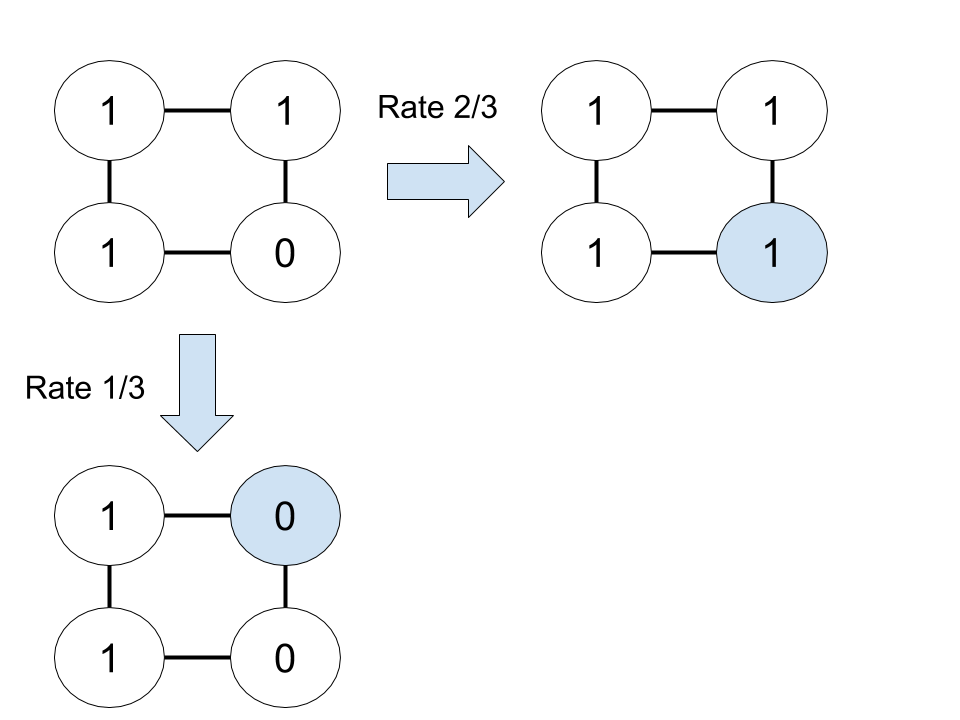
\includegraphics[width=.80\textwidth]{figures/voter_model_config_example.png}
\end{figure}
\end{frame}

\begin{frame}
The transition rates have the following properties:
\begin{enumerate}
    \item $q(\eta, \eta_x) = 0$ for each $x \in \Z^d$ if $\eta \equiv 0$ or $\eta \equiv 1$
    \item $q(\eta, \eta_x) = q(\zeta, \zeta_x)$ for every $x \in \Z^d$ if $\eta(y) + \zeta(y) = 1$ for all $y \in \Z^d$. That is, the dynamics of the system are not changed by interchanging 1 and 0.
    \item On a finite graph eventually the graph will be either $\equiv 0$ or $\equiv 1$.
\end{enumerate}
\end{frame}

\begin{frame}{Voter Model Simulation on $Z$}
\begin{figure}[H]
  \centering
    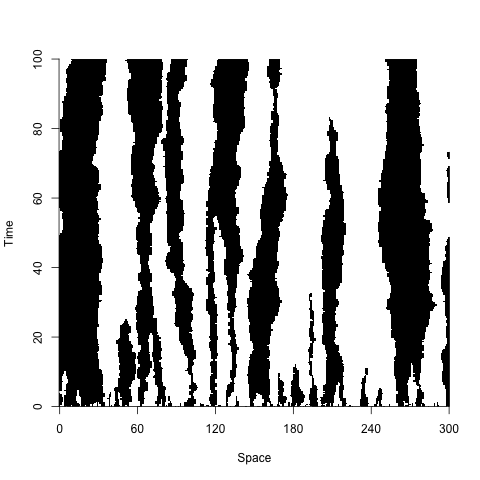
\includegraphics[width=.6\textwidth]{figures/voter_simulation_1d_300.png}
   \caption{Simulation for voter model with periodic boundary conditions on length 300 subset of $\Z$}
  \label{fig:voter_sim_1d_torus.png}
\end{figure}
\end{frame}

% \begin{frame}{Voter Model Simulation on $Z^2$}
% \begin{figure}[H]
%   \centering
%     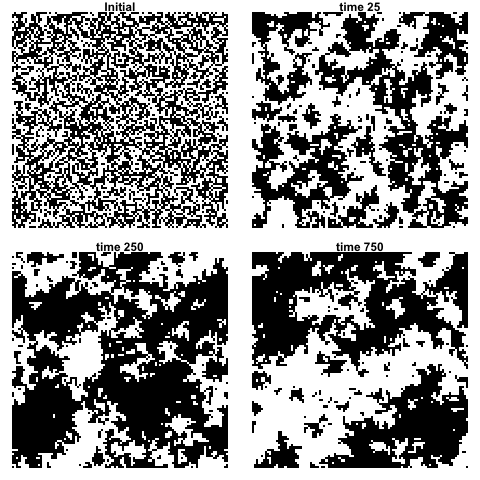
\includegraphics[width=.6\textwidth]{figures/voter_simulation_torus_100.png}
%   \caption{Simulation for voter model with periodic boundary conditions on $100 \times 100$ grid.}
%   \label{fig:voter_sim_2d_torus.png}
% \end{figure}
% \end{frame}

\begin{frame}{Voter Model on Complete Graph}
    \begin{itemize}
        \item In the complete graph each node in a configuration is connected to all of the others
        \item Project a configuration $\eta$ to the minimum number of 1's in $\eta$ and $1 - \eta$.
        $$
        \eta \mapsto \min\left(|\{x : \eta(x) = 1\}|, |\{x : \eta(x) = 0\}|  \right)
        $$
        \item We then have a new Markov chain with $\lfloor n/2 \rfloor + 1$ projected states.
        \item Denote the complete graph with $i$ nodes as $K_i$
    \end{itemize}
\end{frame}

\begin{frame}{Voter Model Simulation on Complete Graph}
\begin{figure}[H]
  \centering
    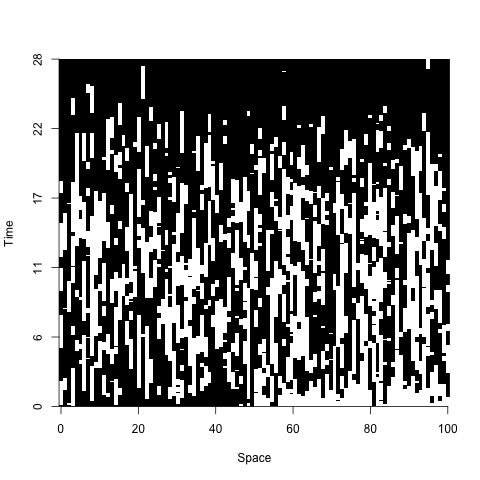
\includegraphics[width=.6\textwidth]{figures/voter_simulation_1d_complete_split_100.png}
   \caption{Simulation for voter model on a complete graph with 100 nodes. The initial configuration is split with half 1's and half 0's.}
  \label{fig:voter_sim_1d_complete.png}
\end{figure}
\end{frame}

\begin{frame}{Voter Model Projection $n = 2$}
    \begin{figure}[H]
  \centering
    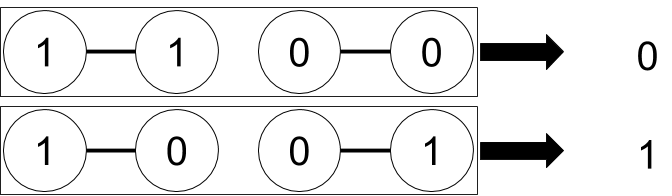
\includegraphics[width=.8\textwidth]{figures/voter_model_proj_2.png}
   \caption{Projection for voter model with $n = 2$}
  \label{fig:voter_sim_1d_torus.png}
\end{figure}
\end{frame}

\begin{frame}{Voter Model Projection $n = 3$}
    \begin{figure}[H]
  \centering
    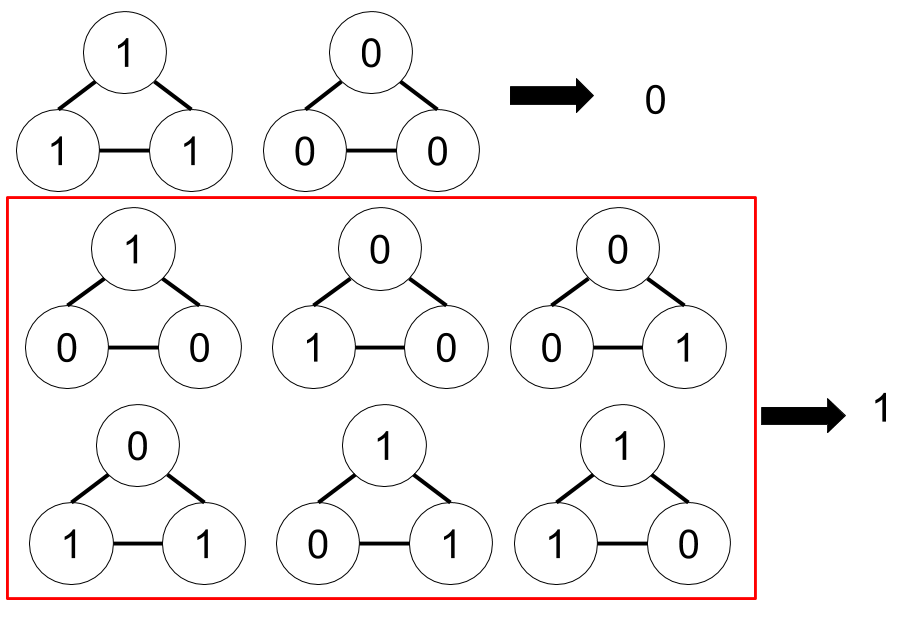
\includegraphics[width=.8\textwidth]{figures/voter_model_proj_3.png}
   \caption{Projection for voter model with $n = 3$}
  \label{fig:voter_sim_1d_torus.png}
\end{figure}
\end{frame}

\begin{frame}{Voter Model Complete Graph $n = 2,3$}
    \begin{itemize}
        \item A complete graph (or a cycle) with $n = 2$ or $n = 3$.
        \item Two projected states, $\{0,1\}$
        \item When $n = 2$, both nodes can change from $1 \to 0$, and $0 \to 1$, each at a rate of $1$ for a total rate of $2$.
        \item When $n = 3$, then the one node that is different from the others can switch to agree with the others. It is connected to 2 other nodes each with a rate of $1/2$ for a total rate of 1.
    \end{itemize}
\end{frame}

\begin{frame}{Voter Model Complete Graph $n = 4$}
\begin{itemize}
    \item The state space in the projected four node voter model is $\{0,1,2\}$.
    % \item When we are in state 2 all nodes can switch from 1 to 0 or 0 to 1 to go to state 1.
    % \item Each of these switch at a rate of $2 \cdot 1/(4 - 1) = 2/3$ since they are connected to 2 other nodes with the opposite value. Thus, the rate from $2 \to 1$ is $8/3$.
    \item The rates are summarized in the form of the infinitesimal generator matrix

$$
Q_{K_4} = \begin{blockarray}{cccc}
    & 2 & 1 & 0\\
    \begin{block}{c|ccc}
        \cline{2-4}
        2 & -\frac{8}{3} & \frac{8}{3} & 0 \\
        1 & 1 & -2 & 1\\
        0 & 0 & 0 & 0\\
    \end{block}
\end{blockarray}
$$
\end{itemize}
\end{frame}

\begin{frame}{Phase Type Distribution Voter Model $n = 4$}
Now we can use the Phase-type distribution theory.
Let
    \begin{align*}
    \mathbf{S} &= \begin{bmatrix}
    -\frac{8}{3} & \frac{8}{3}\\
    1 & -2\\
    \end{bmatrix}\\
    \mathbf{S}_0 &= (0, 1)^T
\end{align*}

The diagonalization of $S$ is
$$
\mathbf{S} = \frac{1}{10} \begin{bmatrix}
    -2 & 4/3\\
    1 & 1
\end{bmatrix} \operatorname{diag}(-4x, - \frac{2}{3} x)
 \begin{bmatrix}
    -3 & 4\\
    3 & 6
\end{bmatrix}
$$
\end{frame}

\begin{frame}{Phase Type Distribution Voter Model $n = 4$}
    Let $(\alpha_2, \alpha_1)$ be the probability of starting in state 2 and 1 respectively.
    The density of the absorption time $\tau_{K_4}$ is given as
\begin{align*}
    f_{K_4}(x) &= (\alpha_2, \alpha_1) \exp(x\mathbf{S}) \mathbf{S}_0\\
    &= \frac{1}{5} \left[ \alpha_2 \left( -4 e^{-4x} + 4 e^{-\frac{2}{3} x} \right) + \alpha_1 \left( 2 e^{-4x} + 3 e^{-\frac{2}{3} x} \right) \right]\\
&= \frac{1}{5} \left[ (-4 \alpha_2 + 2 \alpha_1) e^{-4x} + (4 \alpha_2 + 3 \alpha_1) e^{-\frac{2}{3} x}\right]
\end{align*}
\end{frame}

\begin{frame}{Phase Type Distribution Voter Model $n = 4$}
    The expected value of $\tau_{K_4}$ is then
\begin{align*}
    E[\tau_{K_4}] &= -1 (\alpha_2, \alpha_1) \mathbf{S}^{-1} (1, 1)^T\\
    &= \frac{1}{8} (\alpha_2, \alpha_1) \begin{bmatrix}
    6 & 8\\
    3 & 8
    \end{bmatrix} (1,1)^T\\
    &= \frac{7}{4} \alpha_2 + \frac{11}{8} \alpha_1
\end{align*}
\end{frame}

\begin{frame}{Phase Type Distribution Voter Model $n = 4$}
    \begin{figure}[H]
  \centering
    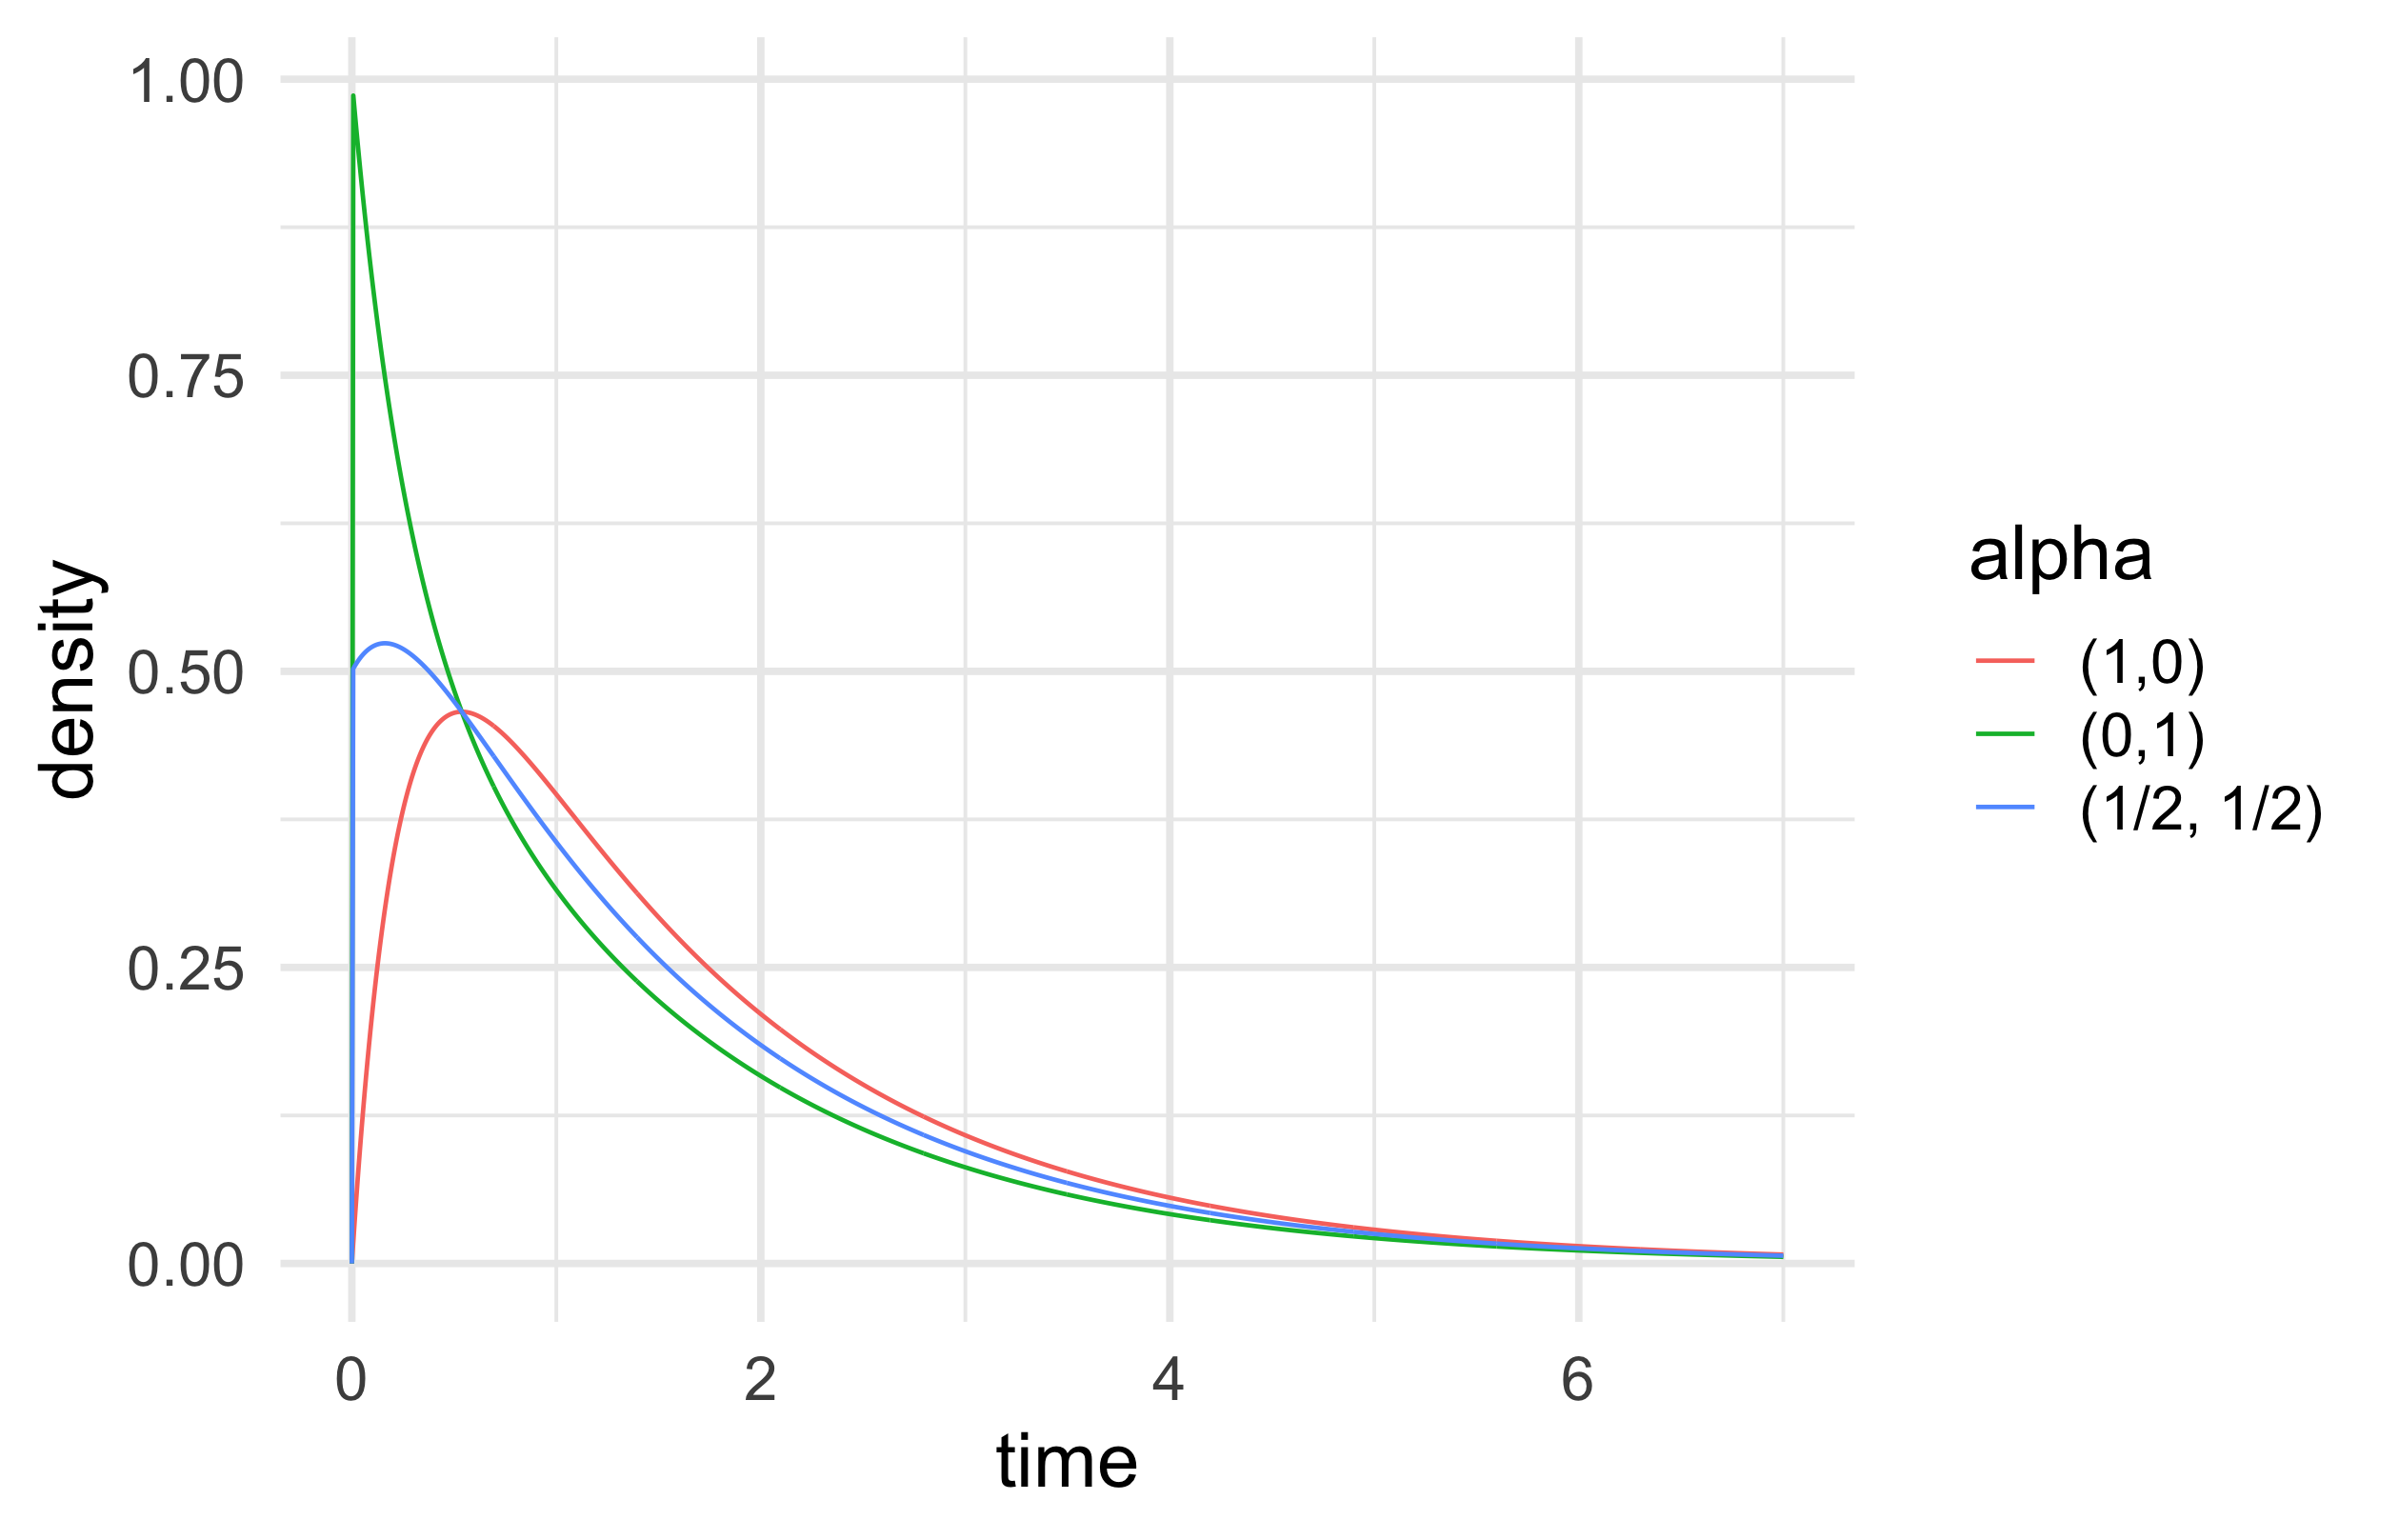
\includegraphics[width=.9\textwidth]{figures/voter_density_c4.png}
   \caption{Density of the absorption time for the voter model on the complete graph with four nodes, $K_4$.}
  \label{fig:voter_density_c4}
\end{figure}
\end{frame}

\begin{frame}{Phase Type Distribution Voter Model $n$ nodes}
    \begin{itemize}
        \item If $n$ is even, then let $k = n / 2$ and if $n$ is odd then let $k = (n - 1)/2$.
        \item We have $\{0,\ldots, k\}$ projected states.
    \end{itemize}

The rates are summarized follows:
\begin{align*}
    i \to i - 1 &= \begin{cases}
        0 & i = 0\\
        \frac{nk}{n - 1}  & i = k, n \text{ even}\\
        \frac{k (n - k)}{n - 1} & i = k, n \text{ odd}\\
        \frac{i (n - i)}{n - 1}  & i \in \{1,\ldots, k - 1\}
    \end{cases}\\
    i \to i + 1 &= \begin{cases}
        0 & i \in \{0, k\}\\
        \frac{i (n - i)}{n - 1}  & i \in \{1,\ldots, k - 1\}
    \end{cases}
\end{align*}
The embedded discrete Markov chain is just a simple random walk on $\{0,\ldots, k\}$ where 0 is absorbing and $k$ reflects back.
\end{frame}

\begin{frame}{Phase Type Distribution Voter Model $n$ nodes}
   Let $N_1, N_2, \ldots, N_k$ be the number of visits to states $1, 2, \ldots, k$ respectively, which are geometrically distributed.
   
$$
E[N_i] = \begin{cases}
    2i & 0 < i < k\\
    k & i = k
\end{cases}
$$   

For all $i = 1,2,\ldots, N_i$ and $j = 1,2,\ldots, k$, let $X_i^{(j)}$ be i.i.d random variables representing the exponential waiting time at each state.


\end{frame}

\begin{frame}{Phase Type Distribution Voter Model $n$ nodes}
Assuming that we start in state $k$ we can represent $\tau_{K_n}$ as random sums
$$
    \tau_{K_n} = \sum_{i = 1}^{N_k} X_i^{(k)} + \sum_{i = 1}^{N_{k - 1}} X_i^{(k - 1)} + \cdots + \sum_{i = 1}^{N_1} X_i^{(1)}
$$
Where $N_j$ is independent of $(X_i^{(j)})$ for each $j$ but these random sums are not independent of each other
\end{frame}

\begin{frame}{Phase Type Distribution Voter Model $n$ nodes}
    \begin{align*}
    E[\tau_{K_n}] &= E\left[\sum_{i = 1}^{N_k} X_i^{(k)} + \sum_{i = 1}^{N_{k - 1}} X_i^{(k - 1)} + \cdots + \sum_{i = 1}^{N_1} X_i^{(1)}\right]\\
    &= E[N_k] E[X^{(k)}] + E[N_{k - 1}] E[X^{(k - 1)}] + \cdots + E[N_1]E[X_i^{(1)}]\\
    &= k E[X^{(k)}] + \sum_{j = 1}^{k - 1} \frac{n - 1}{(n - j)}\\
    &= \begin{cases}
    (n - 1) \left[H_{n} - H_{n - k}\right] & n \text{ even}\\
    (n - 1) \left[H_{n - 1} - H_{n - k - 1}\right] & n \text{ odd}
    \end{cases}
    \end{align*}
Where $H_n$ is the $n$th harmonic number $H_n = \sum_{k = 1}^n \frac{1}{k}$

For large $n$, $E[\tau_{K_n}] \approx ln(2) (n - 1)$ since $\lim_{n \to \infty} [H_n - ln(n)] = \gamma = 0.577$
\end{frame}


\section{Contact Process}

\begin{frame}
\begin{itemize}
    \item The contact process $(\eta_t)$, is a continuous-time Markov chain
    \item Let $G = (V,E)$ be a graph with finite or countably infinite vertices
    \item The state space is $S = \{0,1\}^V$
    \item Infection rate $\lambda$
    % \item Each 1 on the graph waits an exponentially distributed random time with rate 1 and then becomes a 0.
    % \item Every 0 waits an exponentially distributed random time with rate $k \lambda$, where $k$ is the number of edges shared with a 1.
    % \item Project the contact process to the number of ones in the configuration
    \item Denote the extinction/absorption time as $\tau_{G}$
    \item If $S$ is finite, the transition rates can be described as follows
$$
q(\eta, \eta_x) = \begin{cases}
    1 & \text{if } \eta(x) = 1\\
    \lambda |\{ (x,y) \in E : \eta(y) = 1\}| & \text{if } \eta(x) = 0
\end{cases}
$$
\end{itemize}

\end{frame}

\begin{frame}{Contact Process Supercritical Case}
    \begin{figure}[H]
  \centering
    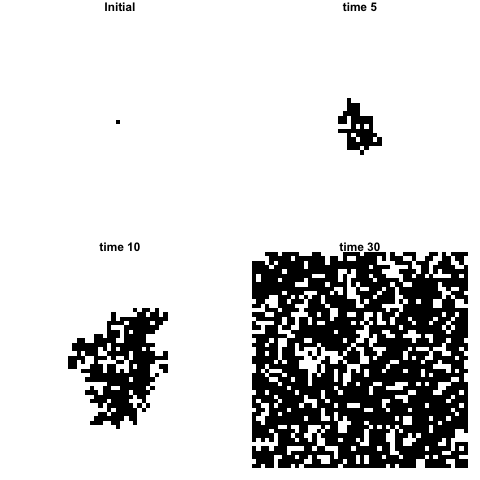
\includegraphics[width=.65\textwidth]{figures/contact_simulation_torus_25.png}
   \caption{Simulation for contact process with $\lambda = 4$ and periodic boundary conditions on $50 \times 50$ grid.}
  \label{fig:contact_sim_torus_above_crit.png}
\end{figure}
\end{frame}

\begin{frame}{Contact Process Subcritical Case}
\begin{figure}[H]
  \centering
    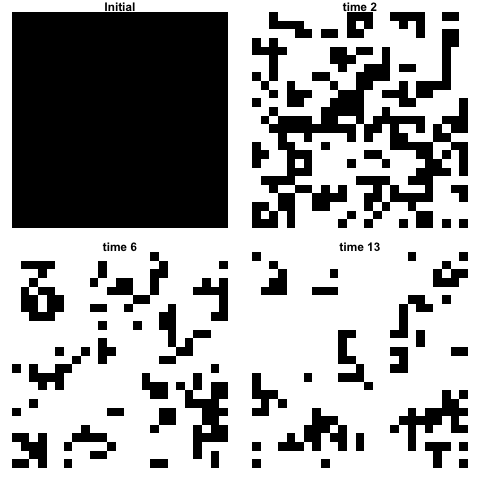
\includegraphics[width=.65\textwidth]{figures/contact_simulation_torus_25_below_crit.png}
   \caption{Simulation for contact process with $\lambda = 0.25$ on $\{0,1\}^{(\Z/50) \times (\Z/50)}$.}
  \label{fig:contact_sim_torus_below_crit.png}
\end{figure}
\end{frame}

\begin{frame}{Contact process 2 nodes}
The contact process with infection rate $\lambda$ on the finite graph with two nodes and one edge between them has the following transition rates

\begin{align*}
    1 &\to 0 \text{ at rate } 1\\
    0 &\to 1 \text{ at rate } \begin{cases}
        \lambda & \text{ if neighbor is 1}\\
        0 & \text{ otherwise}
    \end{cases}
\end{align*}

\begin{figure}
    \centering
   \begin{tikzpicture}[start chain = going right,
   -Triangle, every loop/.append style = {-Triangle}]
   \node[state, on chain]  (2) {2};
   \node[state, on chain]  (1) {1};
   \node[state, on chain]  (0) {0};

   \draw (2) edge[bend left] node[yshift=3mm]{$2$} (1);
   \draw (1) edge[bend left] node[yshift=-3mm]{$\lambda$}(2);
   \draw (1) edge[left] node[xshift=3mm, yshift=-3mm]{$1$} (0);

\end{tikzpicture}
\end{figure}

\end{frame}

\begin{frame}{Contact Process $n = 2$ Phase-type distribution}
$$
    \mathbf{S} = \begin{pmatrix}
        -2 & 2\\
        \lambda & - (1 + \lambda)
    \end{pmatrix}, \quad
    \mathbf{S}_0 = \begin{pmatrix}
        0\\
        1
    \end{pmatrix}, \quad
    \boldsymbol{\alpha} = \begin{pmatrix}
    1 & 0
    \end{pmatrix}
$$
then
\begin{align*}
 f(x; \lambda) &= \boldsymbol{\alpha} \exp(x \mathbf{S}) \mathbf{S}_0\\
 &= \frac{2}{C} \left( e^{\frac{1}{2}(-3 - \lambda + C) x} - e^{\frac{1}{2}(-3 - \lambda - C) x} \right)
\end{align*}
where
$$
C = \sqrt{\lambda^2 + 6 \lambda + 1}
$$
\end{frame}

\begin{frame}{Contact process 2 node Phase-type density}
\begin{figure}[H]
  \centering
    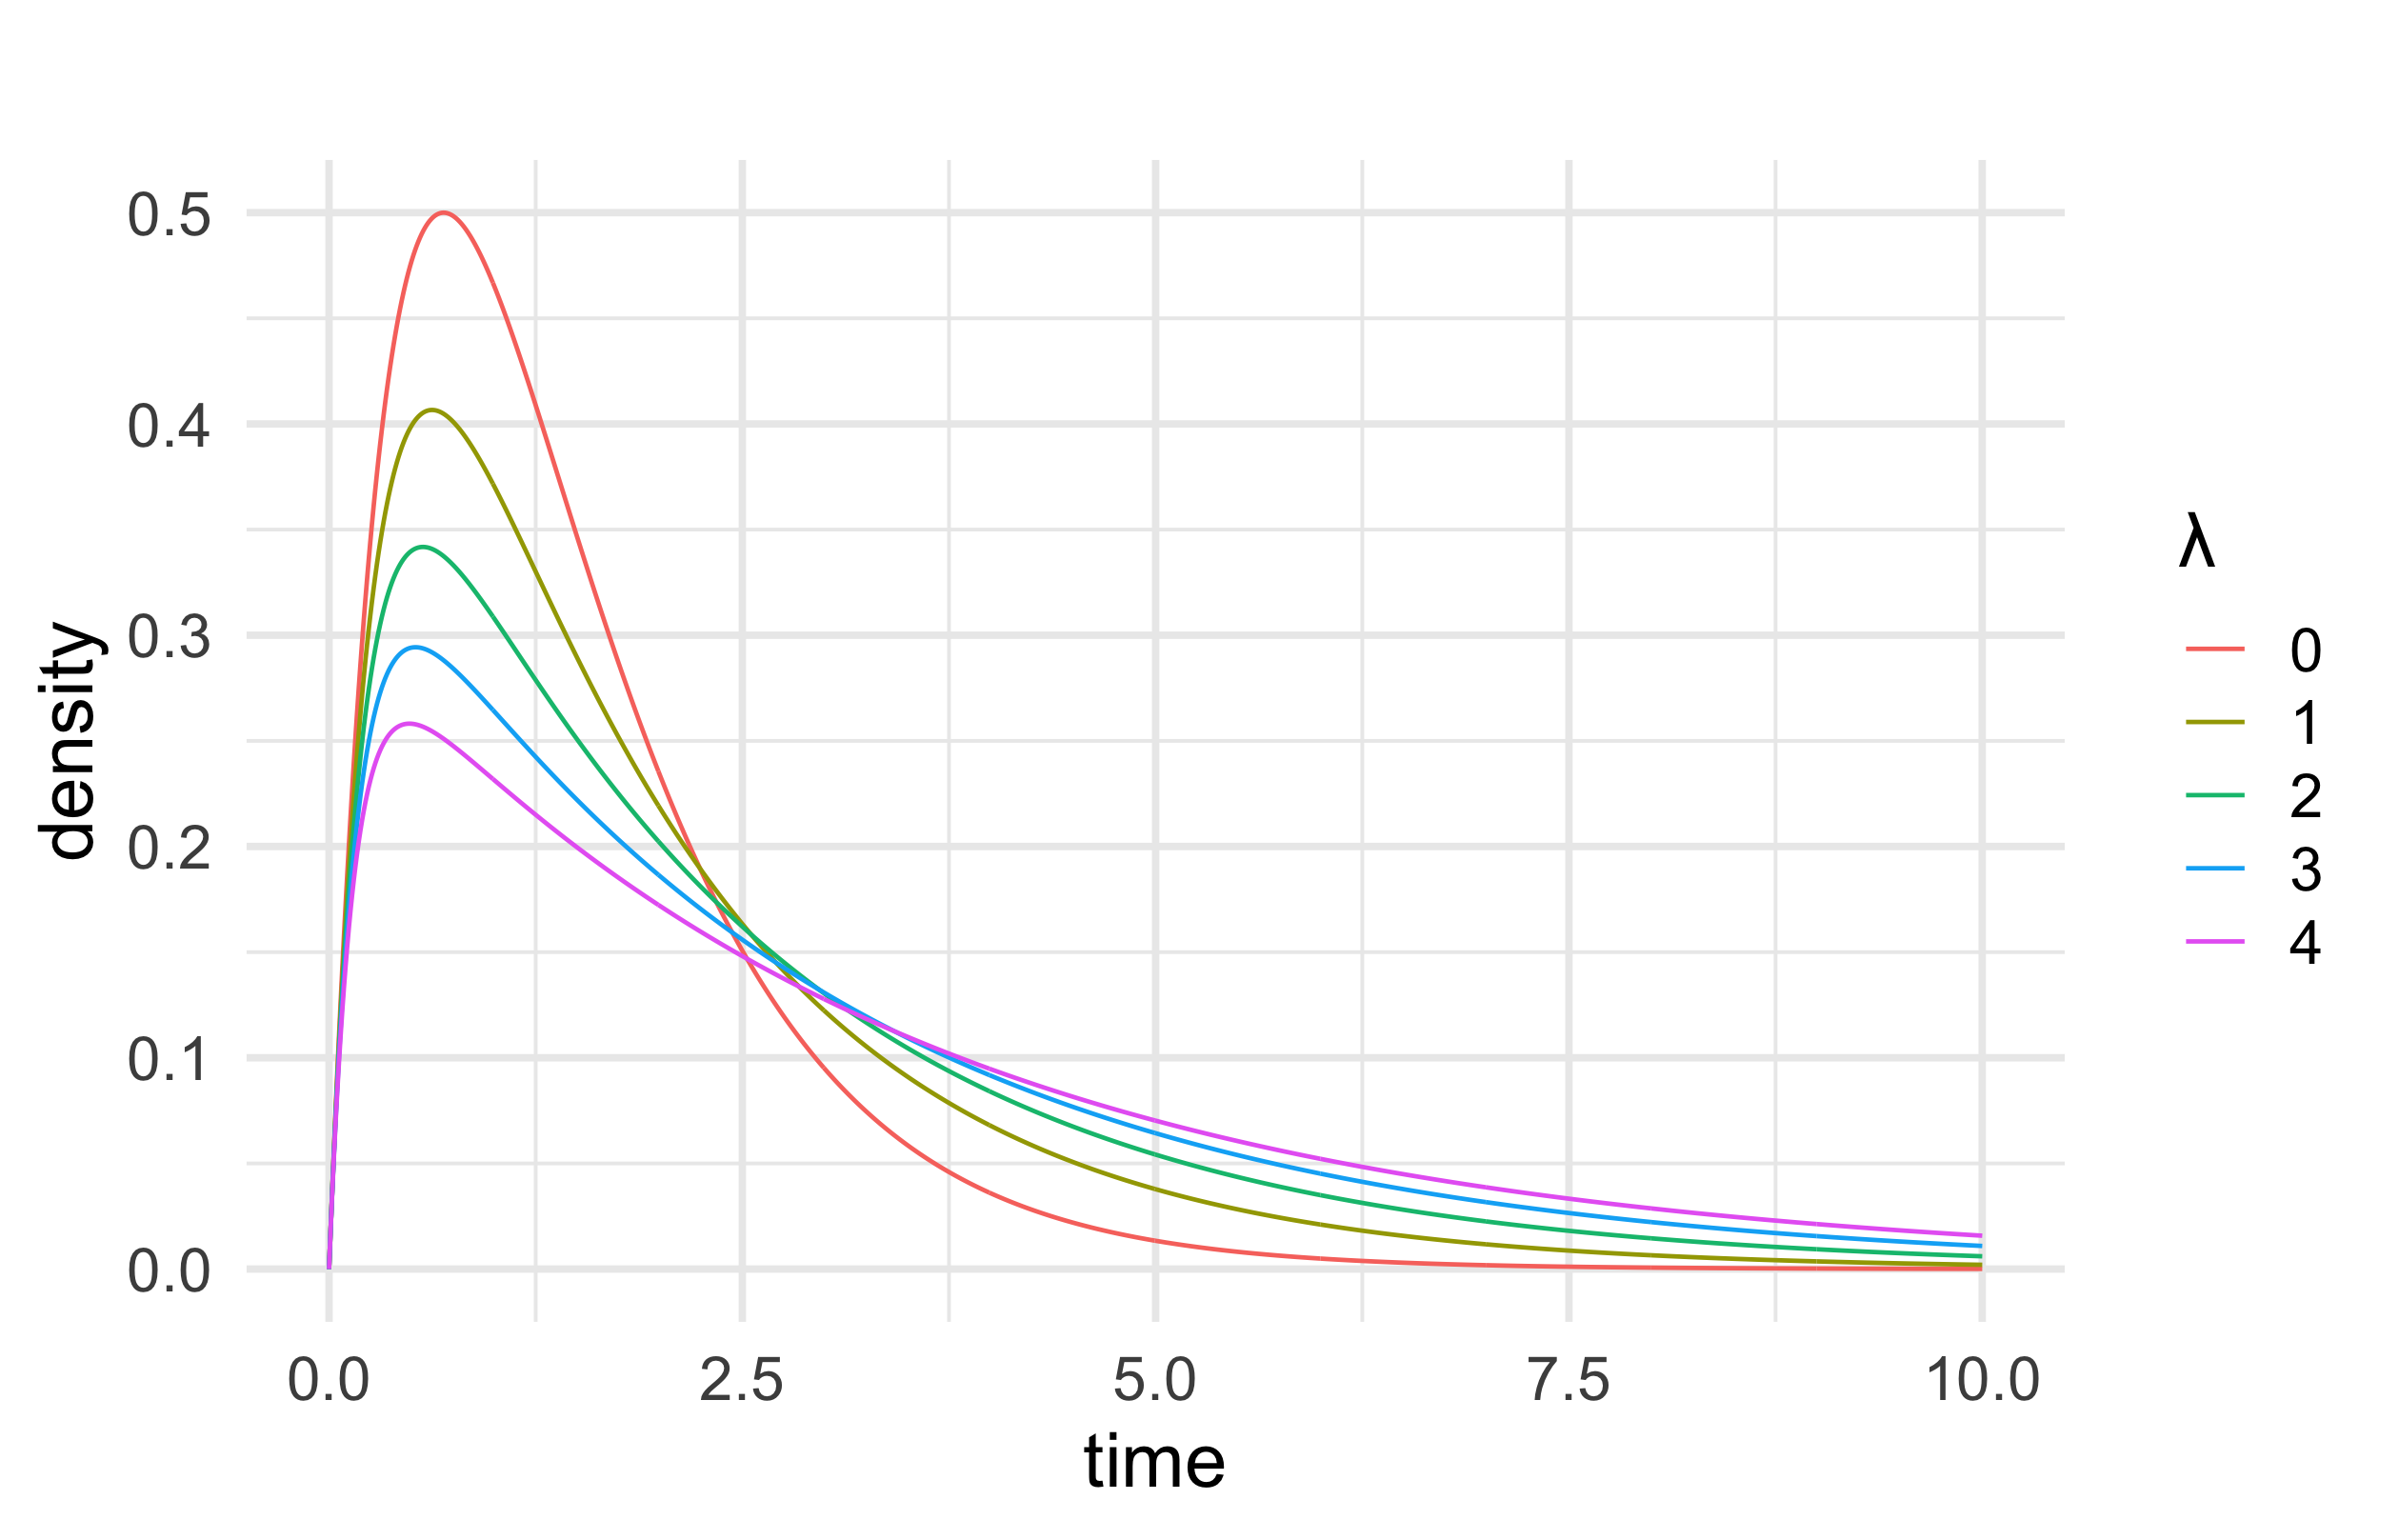
\includegraphics[width=.80\textwidth]{figures/complete_2_contact_phase_densities.png}
   \caption{Density functions for $\tau_{K_2}$ for $\lambda = 0, 1, 2, 3, 4$}
  \label{fig:contact_2_phase_densities}
\end{figure}
\end{frame}

\begin{frame}{Contact process 2 nodes}
We can express $\tau_{K_2}$ as a random sum
$$
\tau_{K_2} = \sum_{i = 1}^N (X_i + Y_i)
$$
where 
\begin{itemize}
    \item $X_1, X_2, \ldots$ be i.i.d random variables with
$X_i \sim \exp(2)$ for the waiting time at state 2
    \item $Y_1, Y_2, \ldots$ with  $Y_i \sim \exp(1 + \lambda)$ (independent of $(X_n)$
    \item $N$ is independent of both $(X_n)$ and $(Y_n)$
    \item $\tau_{K_2} \Rightarrow \infty$ as $\lambda \to \infty$
\end{itemize}
\end{frame}

\begin{frame}{Limiting Distribution}
$$
\tau_{K_2} = \sum_{i = 1}^N X_i +  \sum_{i = 1}^N  Y_i
$$
where
$$
X_i \sim \exp(2),\quad Y_i \sim \exp(1 + \lambda),\quad N \sim \operatorname{Geom}\left(\frac{1}{1 + \lambda}\right)
$$

\begin{align*}
    \sum_{i = 1}^N X_i &\sim \exp\left( \frac{2}{1 + \lambda} \right) && \frac{2}{1 + \lambda}\sum_{i = 1}^N X_i \sim \exp( 1 ) \\
    \sum_{i = 1}^N Y_i &\sim \exp( 1 ) &&\frac{2}{1 + \lambda}\sum_{i = 1}^N Y_i \sim \exp \left( \frac{1 + \lambda}{2} \right) \Rightarrow 0
\end{align*}
as $\lambda \to \infty$. Therefore
$$
\frac{2}{1 + \lambda} \tau_{K_2} \Rightarrow \exp(1) \text{ as } \lambda \to \infty
$$

\end{frame}

\begin{frame}{Contact process 3 node phase-type density}
\begin{figure}[H]
  \centering
    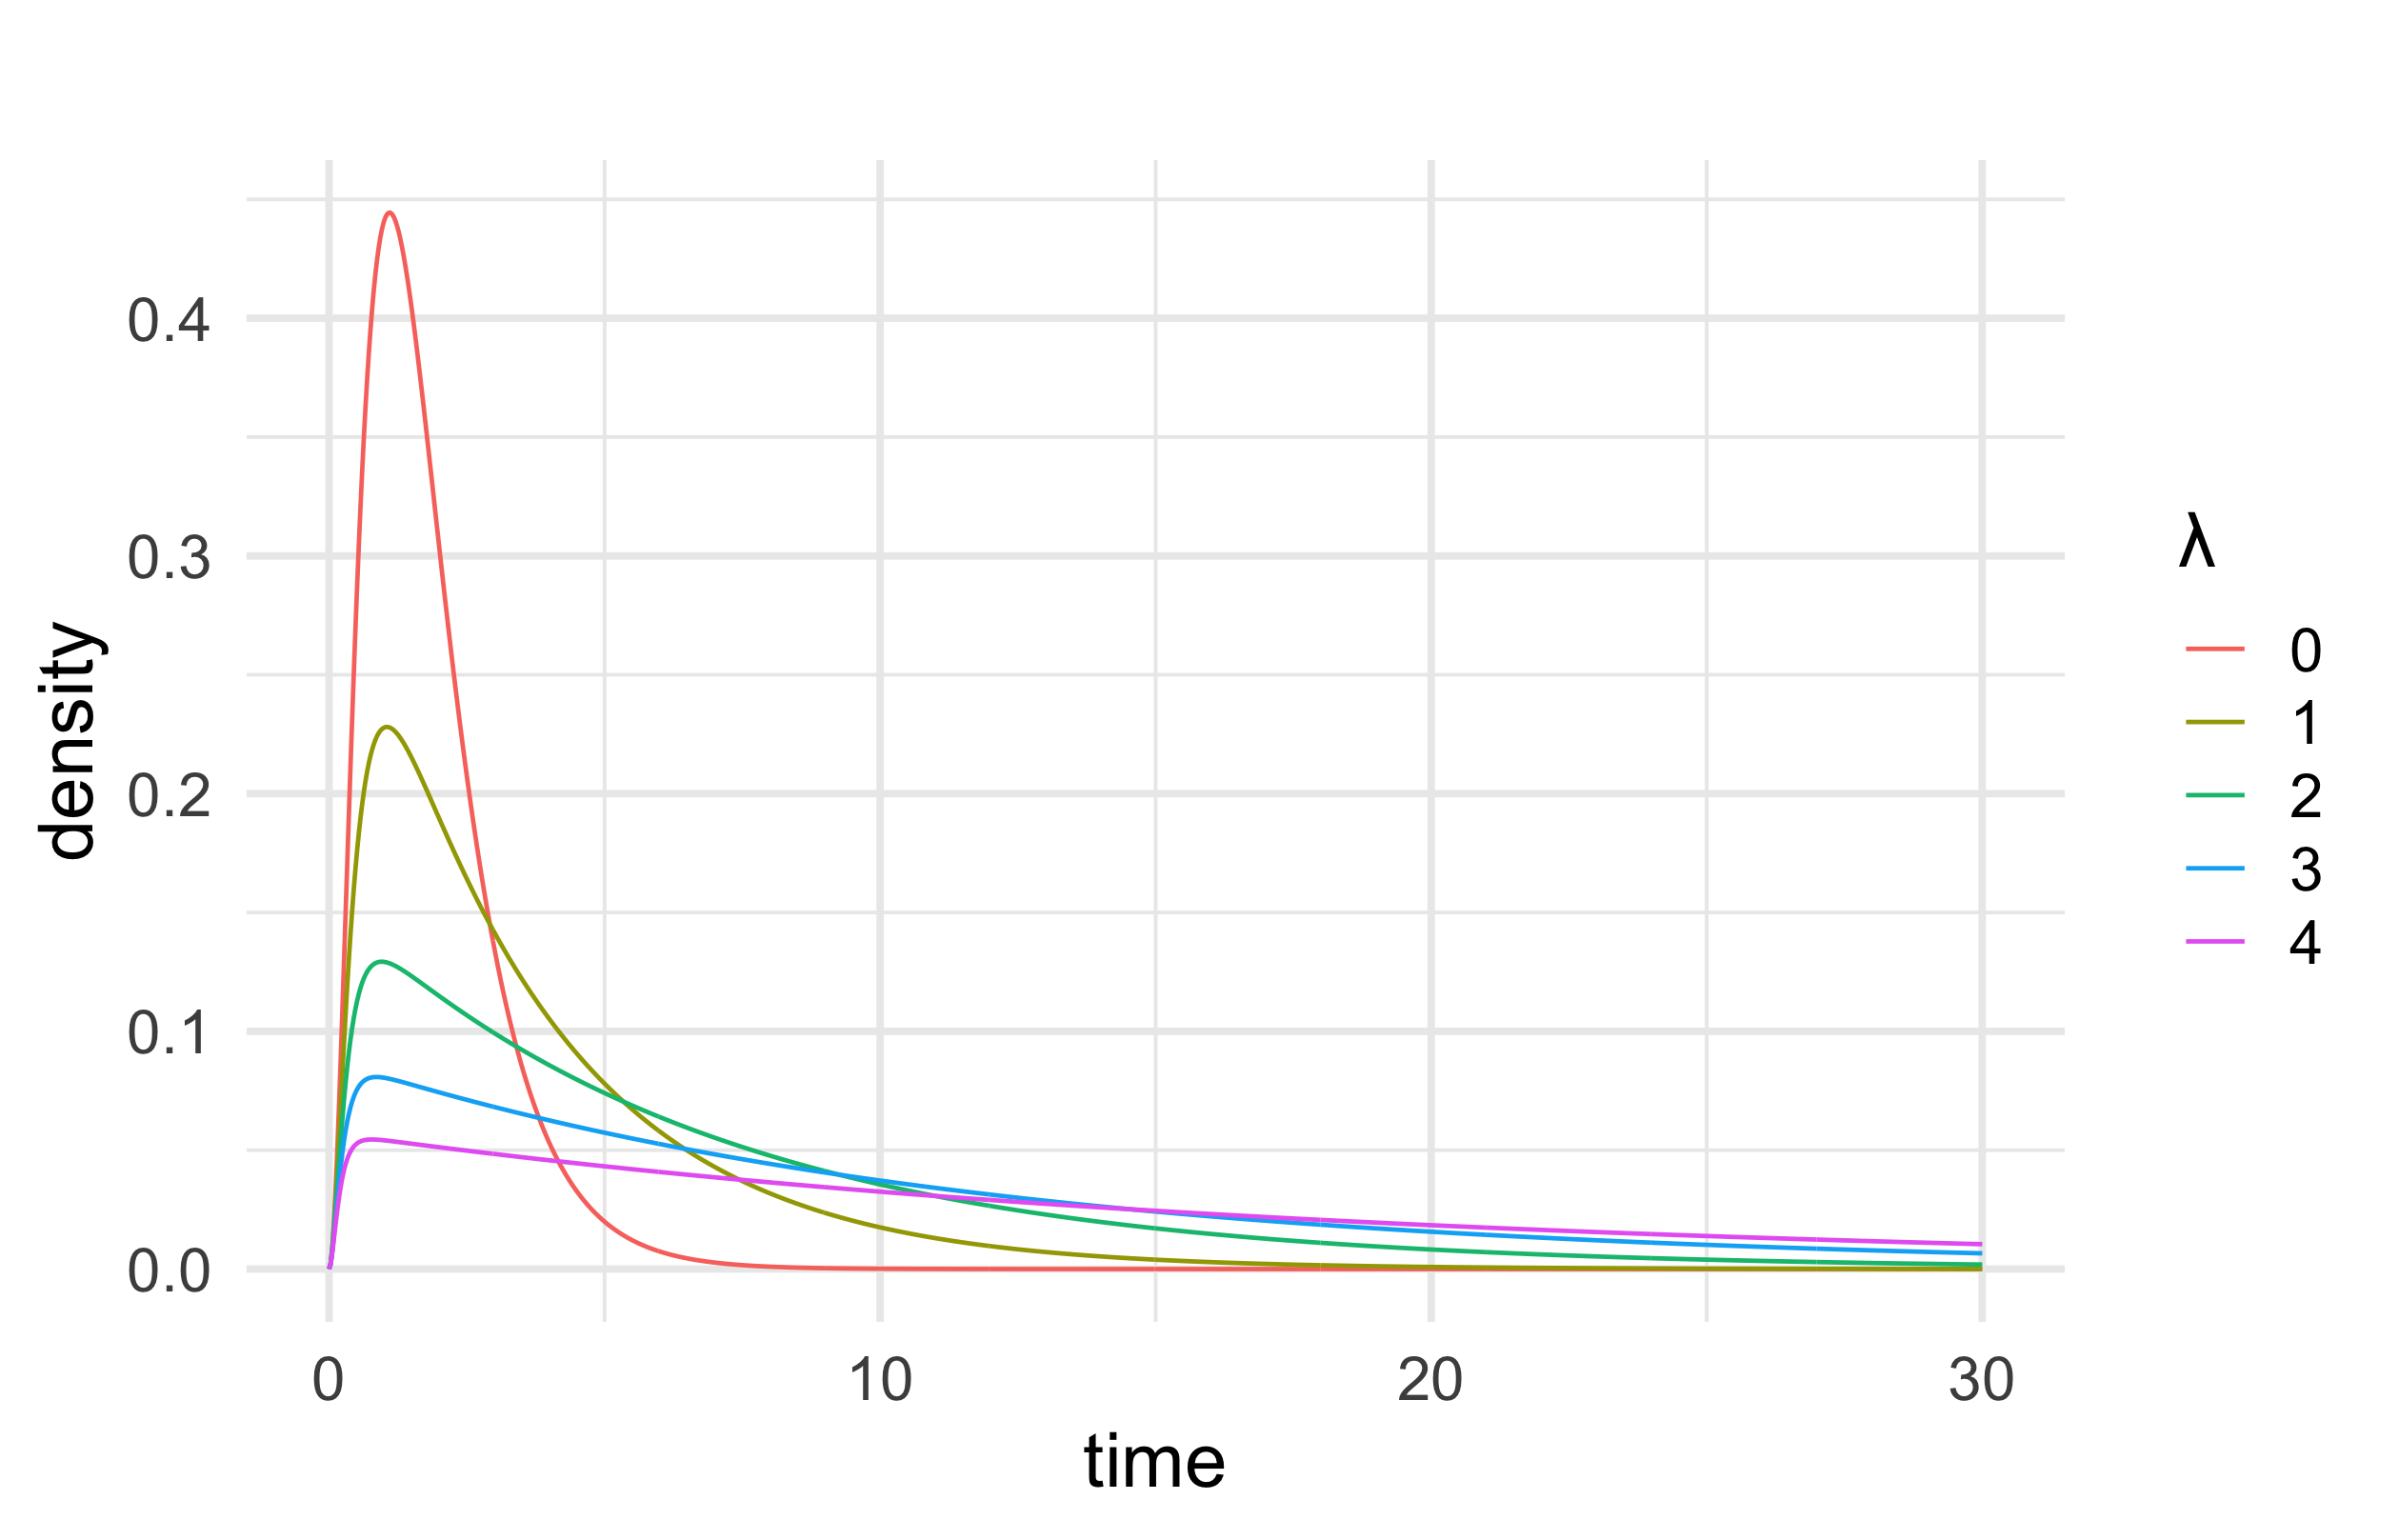
\includegraphics[width=.80\textwidth]{figures/complete_3_contact_phase_densities.png}
   \caption{Density functions for $\tau_{K_3}$ for $\lambda = 0, 1, 2, 3, 4$ on the complete three node contact process}
  \label{fig:contact_3_phase_densities}
\end{figure}
\end{frame}

\begin{frame}{Contact process $n$ node}
    \begin{figure}[H]
    \centering
   \begin{tikzpicture}[
   start chain = going right,
   -Triangle,
   every loop/.append style = {-Triangle}]
   \node[state, on chain]  (n) {n};
   \node[state, on chain]  (n1) {n - 1};
   \node[state without output/.append style={draw=none}, on chain]  (dots1) {...};
   \node[state, on chain]  (2) {2};
   \node[state, on chain]  (1) {1};
   \node[state, on chain]  (0) {0};

   \draw (n) edge[bend left] node[yshift=3mm]{$n$} (n1);
   \draw (n1) edge[bend left] node[yshift=-3mm]{$1 (n - 1) \lambda$}(n);


   \draw (n1) edge[left] node[xshift=3mm, yshift=-3mm]{} (dots1);

   \draw (dots1) edge[left] node[xshift=3mm, yshift=-3mm]{} (2);

  \draw (2) edge[bend left] node[yshift=3mm]{$2$} (1);
   \draw (1) edge[bend left] node[yshift=-3mm]{$(n - 1)1 \lambda$}(2);

  \draw (1) edge[left] node[yshift=3mm]{$1$} (0);
\end{tikzpicture}
    \caption{Transition rates for N node complete contact process}
    \label{fig:complete_contact_n_node_rates}
\end{figure}

\begin{align*}
    i \to i - 1 &= \begin{cases}
        0 & i \in 0\\
        i & i \in \{1,\ldots, n\}
    \end{cases}\\
    i \to i + 1 &= \begin{cases}
        0 & i = i \in \{0, n\}\\
        i(n - i) \lambda & i \in \{1,\ldots, n-1\}
    \end{cases}
\end{align*}
\end{frame}

\begin{frame}{Contact Process Limiting Distribution}
    Let $\tau_{K_n}$ be the time until we reach state zero.
Now let $N_1, N_2, \ldots, N_n$ be the number of visits to states $1, 2, \ldots, n$ respectively.

For all $i = 1,2,\ldots, N_i$, $j = 1,2,\ldots, n$ and let $X_i^{(j)}$ be i.i.d random variables representing the exponential waiting times at each state.

Since we are concerned with the limiting distribution we can instead focus on the rates up to a constant
$$
E[X_i^{(j)}] = E[X^{(j)}] \propto \begin{cases}
  1 & j = n\\
  \frac{1}{1 + \lambda} & j \in \{1,\ldots, k - 1\}\\
\end{cases}
$$
\end{frame}

\begin{frame}{Contact Process Limiting Distribution}
We can again represent $\tau_{K_n}$ as random sums

\begin{equation*}\label{eq:wait_contact_sum}
    \tau_{K_n} = \sum_{i = 1}^{N_n} X_i^{(n)} + \sum_{i = 1}^{N_{n - 1}} X_i^{(n - 1)} + \cdots + \sum_{i = 1}^{N_1} X_i^{(1)}
\end{equation*}

Then the limiting distribution as $\lambda \to \infty$ is
$$
\frac{\tau_{K_n}}{E[N_{n}]E[X^{(n)}]} \Rightarrow \exp(1)
$$
\end{frame}

\begin{frame}[standout]
  Questions?
\end{frame}

%\bibliographystyle{plainnat}
%\bibliographystyle{abbrv}
%\bibliographystyle{abbrvnat}
%\bibliography{references}
\end{document}
